%% LyX 2.2.2 created this file.  For more info, see http://www.lyx.org/.
%% Do not edit unless you really know what you are doing.
\documentclass[english]{article}
\usepackage[T1]{fontenc}
\usepackage[latin9]{inputenc}
\usepackage{float}
\usepackage{graphicx}

\makeatletter

%%%%%%%%%%%%%%%%%%%%%%%%%%%%%% LyX specific LaTeX commands.
%% Because html converters don't know tabularnewline
\providecommand{\tabularnewline}{\\}

\makeatother

\usepackage{babel}
\begin{document}

\part{ELECTRONICA III EJERCICIO 4}

\section{Delay de Propagaci�n - Rise Time - Fall Time}

En esta parte del art�culo se propondr� medir los tiempo de propagaci�n,
rise y fall del 74HC02. A fin de comparar resultados, primero se realizar�n
mediciones en vac�o y luego se repetir�n utilizando el siguiente circuito:

\begin{figure}[H]
\begin{centering}
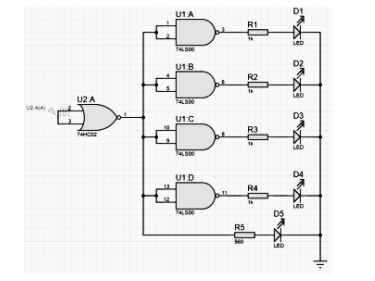
\includegraphics[scale=0.4]{circuitoAmedir.PNG}
\par\end{centering}
\begin{centering}
\caption{Circuito Propuesto a Medir}
\par\end{centering}
\end{figure}


\subsection{Resultados Obtenidos}

Los resultados obtenidos fueron los siguientes:

\begin{table}
\begin{tabular}{|c|c|}
\hline 
Medici�n en Vacio & \tabularnewline
\hline 
\hline 
Tiempo de Rise & 59 ns\tabularnewline
\hline 
Tiempo de Fall & 165 ns\tabularnewline
\hline 
Tiempo de Propagaci�n & 15 ns\tabularnewline
\hline 
\end{tabular}%
\begin{tabular}{|c|c|}
\hline 
Medici�n del Circuito Propuesto & \tabularnewline
\hline 
\hline 
Tiempo de Rise & 51 ns\tabularnewline
\hline 
Tiempo de Fall & 60 ns\tabularnewline
\hline 
Tiempo de Propagaci�n & 18 ns\tabularnewline
\hline 
\end{tabular}

\caption{Mediciones - Resultados Obtenidos}

\end{table}

Estas mediciones se realizaron con una excitaci�n de onda cuadrada
de 500 Hz de frecuencia y con una alimentaci�n de 5 Volts.

Con respecto al tiempo de propagaci�n con el circuito de carga, es
esperable que este sea mayor como lo indic� la medici�n ya que la
carga presenta una componente capacitiva que aletarga la salida medida.

Luego de realizar estas mediciones, se procedi� a aumentar la frecuencia
del generador a 100 KHz y se midi� tensi�n de alimentaci�n. Lo que
se observ� fue que esta no resultaba ser constante. Por consiguiente,
se procedi� a colocar un capacitor de $100nF$ entre los bornes de
la alimentaci�n (entre ``Vcc'' y ``Ground'') a fin de comparar
resultados. A continuaci�n se presentan las dos mediciones de la tensi�n
se alimentaci�n (con capacitor y sin capacitor):

\begin{figure}[H]
\begin{centering}
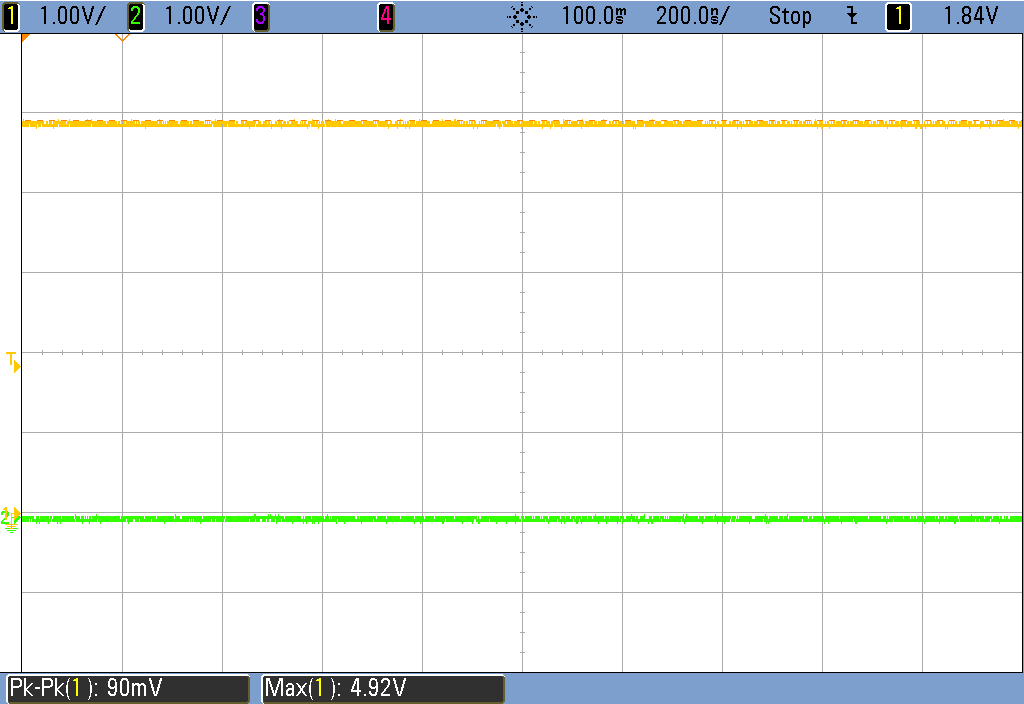
\includegraphics[scale=0.4]{AlimentacionConDesacople}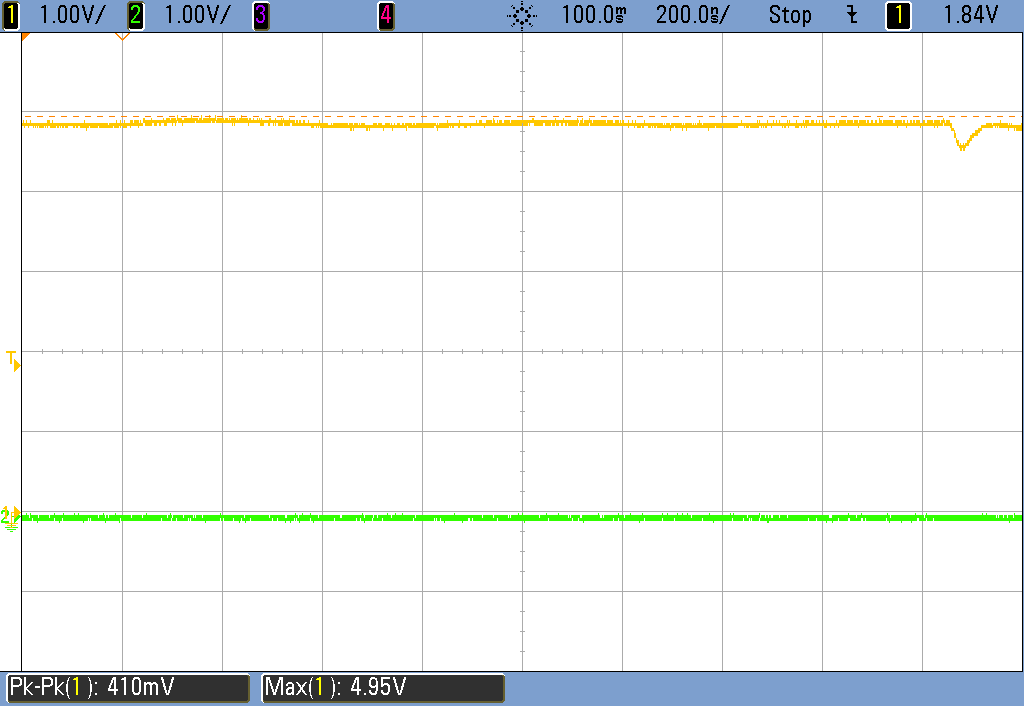
\includegraphics[scale=0.4]{AlimentacionSinDesacople}
\par\end{centering}
\caption{Mediciones - Tensi�n de Alimentaci�n}
\end{figure}

En la medici�n sin capacitor se observa un pico para el cual la tensi�n
de alimentaci�n disminuye, pero que no aparece en la medici�n con
capacitor. Esto se puede explicar debido a que el capacitor contrarresta
las inductancias que existen debido a las conexiones f�sicas y adem�s
el capacitor (si es lo suficientemente grande) es capaz de otorgar
picos de corriente que pueden requerir los transistores del integrado,
sin afectar la tensi�n de alimentaci�n.

Adem�s, al agregar el capacitor se pudo observar un cambio en la forma
de la respuesta de la 74HC02, siendo esta sub-amortiguada con sobre
pico al no colocar el capacitor, pero si se colocaba el capacitor
esta tend�a a ser sobre amortiguada sin sobre pico. A continuaci�n
se muestran dos imagenes que plasman la diferencia de la salida de
la compuerta debida al capacitor de $100nF$:

\begin{figure}[H]

\begin{centering}
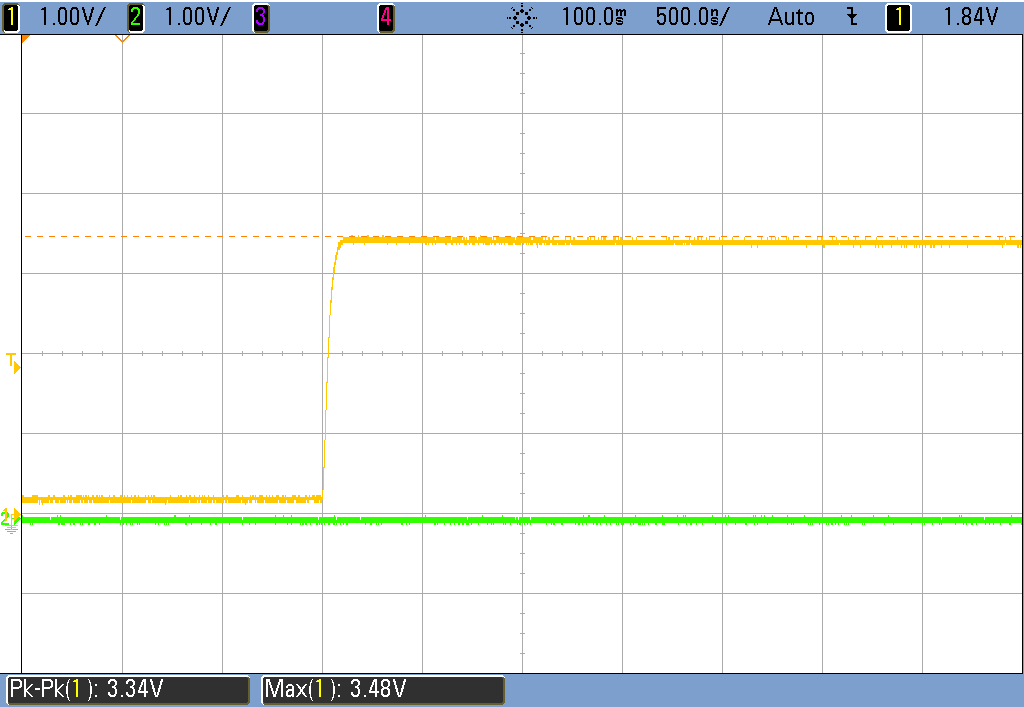
\includegraphics[scale=0.4]{SalidaDeHConDesacople}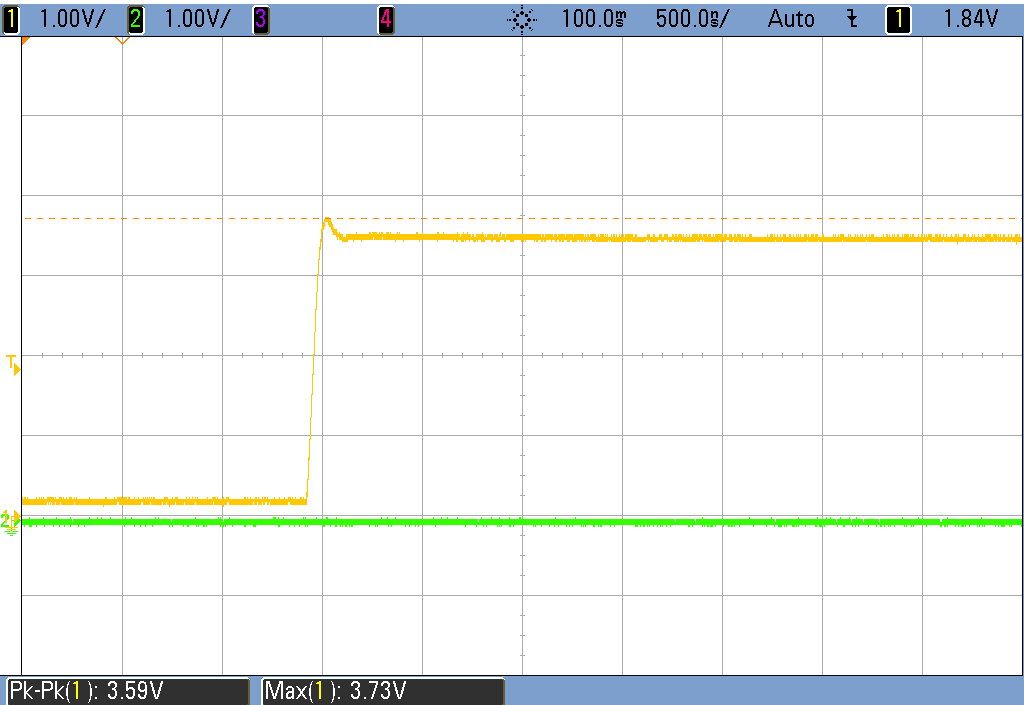
\includegraphics[scale=0.4]{SalidaDeHCSinDesacople}
\par\end{centering}
\caption{Respuesta de 74HC02 Seg�n Acople Capacitivo }

\end{figure}

\end{document}
